\normalfont\normalsize
\chapter{Implementation}

This chapter presents some aspects of the implementation worth mentioning. Some parts of the tasks running on the wireless sensors,
how the algorithm for the scheduler is implemented.
 
\begin{figure}[ht]
\begin{center}
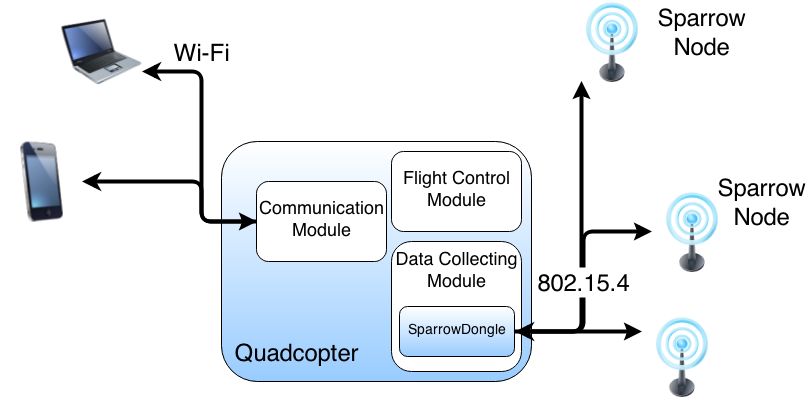
\includegraphics[width=0.9\textwidth]{implementation/organigrama.png}
\end{center}
\caption{\small \itshape{Modules and connections between them and devices}}
\end{figure}

\section{The Debug Module}

The code can be compiled to display debug informations to the console or to supress them entirely. Also, in certain parts of the modules, a wait action is need in order to wait for an action to be executed. Now the delay is set at 100 ms, but it can be easily modiffied to any desired value. 

\lstset{numbers=none, mathescape=true, nolol=false,caption=Data Collection use of mutex,label=lst:task}
\begin{lstlisting}
/* activates/deactivates printf debuf information*/
#define DEBUG_ON 0
/* delay yime in microseconds*/
#define DELAY_US 100000
#define DEBUG_PRINT(a...) { if(DEBUG_ON) printf(a); }
\end{lstlisting}

 

\section{The Data Collecting Module}
 
The module saves the collected data int-o the drones internal memory and pases the data in order to gather certain informations like number of nodes currently connected to the Dongle, de signal strength, if the Dongle is connected etc. This informations are passed to the communication module to provide to the user realtime feedback.


\subsection{Modules intercommunication}

The memory area in which the informations sent to the user are saved is shared between this module and the comunication module. Basically, the way this two modules interract with each other can be compared to the consumer - producer problem, where the Data Collecting Module can be associated with the producer side and the Communication Module with the consumer side.

The main problem consists of deadlocks and data starvation. This is prevent with the use of one mutex that allows only one thread at a time to moddify the informations.

\lstset{numbers=none, mathescape=true, nolol=false,caption=Data Collection use of mutex,label=lst:task}
\begin{lstlisting}
pthread_mutex_lock(&data_lock); 
add_node_data(get_current_timestamp(),read_data + 7);
pthread_mutex_unlock(&data_lock);
\end{lstlisting}

The mutex is used similarly in the Communication Module when it consumes the information.

\lstset{numbers=none, mathescape=true, nolol=false,caption=Data Collection use of mutex,label=lst:task}
\begin{lstlisting}
void add_node_data(long long time_stamp , char *p) {
	int i;
	int id = get_hex(p,2);

	/* the power of the signal calculated in dB */
	int power = -90 + 3* (get_hex(p + 64,2)-1);

	/* creating a file with unique name */
	DEBUG_PRINT("node id %i %i\n",id,power);
	char file_name[100];
	sprintf(file_name, "/node_logs/%lli_%i",file_timestamp,id);

	/* saving the new data at the end of the file */
	FILE *fptr = fopen(file_name,"a");	
	fprintf(fptr,"%s",p);
	fclose(fptr);
	
	/* searching for previous connection of the same node*/
	for(i = 0 ;i < node_nr;i++) {
		if(data[i].id == id) {

			/* timestamp update - node is stil reachable and sending data */
			DEBUG_PRINT("data update\n");
			data[i].time_stamp = time_stamp;
			data[node_nr].power = power;
			return;
		}
	}
	
	/* new node found by the drone */
	DEBUG_PRINT("new node\n");
	data[node_nr].id = id;
	data[node_nr].time_stamp = time_stamp;
	data[node_nr].power = power;
	node_nr ++;
}

\end{lstlisting}



\subsection{Failure proof}

Because the Dongle is connected to an USB port on a machine that has a lot of vibrations, it might desconnect / reconnect for a very short period of time, so this module has been designed  with multiple USB disconnects and reconnects without the need to reset the Drone. This infomation is vital, because you can check if the Dongle is still connected to the dron without the need to inspect it visualy or to connect to a debug terminal.

\lstset{numbers=none, mathescape=true, nolol=false,caption=Data Collection use of mutex,label=lst:task}
\begin{lstlisting}
	while(1) {
		DEBUG_PRINT("attemting connection to Sparrow Dongle\n");
		FILE *ptr = NULL;	
		while(ptr == NULL) {	
			usleep(DELAY_US);
			ptr = fopen("/dev/ttyACM0","r"); 
		}

		dongle_connected = 1;
		DEBUG_PRINT("Sparrow Dongle connected\n");
		char read_data[100]; 
	 
		while(fgets(read_data,100,ptr) != NULL) 
		{
			
			if(check_message_format(read_data)) {
	   	 		pthread_mutex_timedlock(&data_lock,&lock_timeout); 
				add_node_data(get_current_timestamp(),read_data + 7);
				pthread_mutex_unlock(&data_lock);
			}
		}
		dongle_connected = 0;
		fclose(ptr);
		DEBUG_PRINT("Sparrow Dongle Disconnected\n");	
	}
 
\end{lstlisting}
 

\section{The Communication Module}

All the information gathered by the Data Collecting Module would be useless if it cannot be accesed easily. 

This module, as the name suggests, handles the communication of this this crucial information back to the user.

Being a different module, with different attributions than the Data Collecting Module, it has an entire proccess dedicated to it for 3 important reasons:
\begin{itemize}

\item 1. This approach of a module with its one procces allows the modules to run indepently of each other;
\item 2. The Data Collecting Module can collect the data from the Dongle as soon as as it has a new one available;
\item 3. If the Communication Module stops working, the Data Collecting Module continues to save the new informations received. 

\end{itemize}

\subsection{Socket with connection reset}

The communication is done through socket connections listening on port 8888. It accepts only one connection at a time.

If a connected client decides to disconnect before or while a write is performed, a SIGPIPE error signal will be thrown, stopping all the modules. This is prevent by ignoring the signal, forcing the write acction to return a EPIPE, an exiting the this function.

The main proccess will calback the accept\_socket\_connection to reestablish a new connetion.

\lstset{numbers=none, mathescape=true, nolol=false,caption=Data Collection use of mutex,label=lst:task}
\begin{lstlisting}
	// Ignore the SIGPIPE error signal
	signal(SIGPIPE, SIG_IGN);

    struct sockaddr_in server;

    //Create socket
    socket_desc = socket(AF_INET , SOCK_STREAM , 0);
    if (socket_desc == -1)
    {
        DEBUG_PRINT("Could not create socket\n");
		return;
    }
    DEBUG_PRINT("Socket created\n");
     
    //Prepare the sockaddr_in structure
    server.sin_family = AF_INET;
    server.sin_addr.s_addr = INADDR_ANY;
    server.sin_port = htons( 8888 );
     
    //Bind
    if( bind(socket_desc,(struct sockaddr *)&server , sizeof(server)) < 0)
    {
        //print the error message
        DEBUG_PRINT("bind failed. Error\n");
        return ;
    }
    DEBUG_PRINT("bind done\n");
     
    //Listen
    listen(socket_desc , 3);
     

	while(1){
	
		accept_socket_connection();
	
	}
\end{lstlisting}


This function will listen for a new connection. Once a connection is established, it will send information once every DELAY\_US microseconds. The program was configured and tested with a 100 ms wait period that leeds to a ten times per second information update.

This delay is required because:
\begin{itemize}

\item If data is send to often , the socket might be flooded and stop sending the data
\item If there were no delay, it will create an big and useless processor busy state both for the drone and the controlling device.

\end{itemize}

\lstset{numbers=none, mathescape=true, nolol=false,caption=Data Collection use of mutex,label=lst:task}
\begin{lstlisting}
void accept_socket_connection() {
	
    struct sockaddr client;
    char *client_message ;
	int  client_sock , c , read_size;

    //Accept and incoming connection
    DEBUG_PRINT("Waiting for incoming connections...\n");
    c = sizeof(struct sockaddr_in);
     
    //accept connection from an incoming client
    client_sock = accept(socket_desc, (struct sockaddr *)&client, (socklen_t*)&c);
    if (client_sock < 0)
    {
        DEBUG_PRINT("accept failed\n");
       return ;
    }
    DEBUG_PRINT("Connection accepted\n");
     
    //Receive a message from client 
	while(1)    
	{	
		// sleep in order to avoid flooding the socket
		usleep(DELAY_US);
 
		client_message = json_encode();
		// error writing - client disconected
		if (write(client_sock , client_message , strlen(client_message)) != strlen(client_message)) 		{		
			free(client_message);
        	DEBUG_PRINT("Client disconnected \n" );
			// reseting listening procces			
			return;
		}
		free(client_message);
    }
     
    if(read_size == 0)
    {
        DEBUG_PRINT("Client disconnected\n");
        fflush(stdout);
    }
    else if(read_size == -1)
    {
        DEBUG_PRINT("recv failed\n");
    }
} 
\end{lstlisting}
 
\subsection{JSON Encoding of Data}

The data sent is encoded in JSON format, because it is very easy to encode and all devices can decode it.

The informations ecoded are
\begin{itemize}

\item Dongle conection status
\item An array containing node informations
\begin{itemize}

	\item Node unique ID
	\item Last conection time of the node to Dongle
	\item The power of the received signal

	\end{itemize}
\end{itemize}
\lstset{numbers=none, mathescape=true, nolol=false,caption=Data Collection use of mutex,label=lst:task}
\begin{lstlisting}

char * json_encode(){
	int i,msg_index = 0;

	char *client_message = (char*)malloc(3000 * sizeof(char));
	client_message[0]='\0';	

	pthread_mutex_timedlock(&data_lock,&lock_timeout); 
    current_timestamp = get_current_timestamp();
	for(i = 0; i < node_nr;i++) {
		if(current_timestamp - data[i].time_stamp < delta)
		{
			client_message[0]++;
		} else {
			delete_node_data(i);
			i--;
		}
	}
	
	int local_node_nr = node_nr;
	struct node_data local_data[node_nr];	
	memcpy(local_data,data,node_nr * sizeof(struct node_data));
	pthread_mutex_unlock(&data_lock);  
	

	msg_index += sprintf(client_message+msg_index, "{ \"dongle_connected\"=%i ,\"nodes\"=[",dongle_connected);
	
    current_timestamp = get_current_timestamp();
	for(i = 0; i <local_node_nr;i++) {
		if(i > 0 ) {
			msg_index += sprintf(client_message+msg_index, ",");
		}	
		msg_index += sprintf(client_message+msg_index, "{\"node_id\"=%i,\"last_connection_time\"=%i,\"power\"=%i}",local_data[i].id,(int)((current_timestamp - local_data[i].time_stamp)/10),local_data[i].power);	
	}

	msg_index += sprintf(client_message+msg_index, "]}\n");

	return client_message;
}
\end{lstlisting}

\section{Android application modules}


\begin{figure}[ht]
\begin{center}
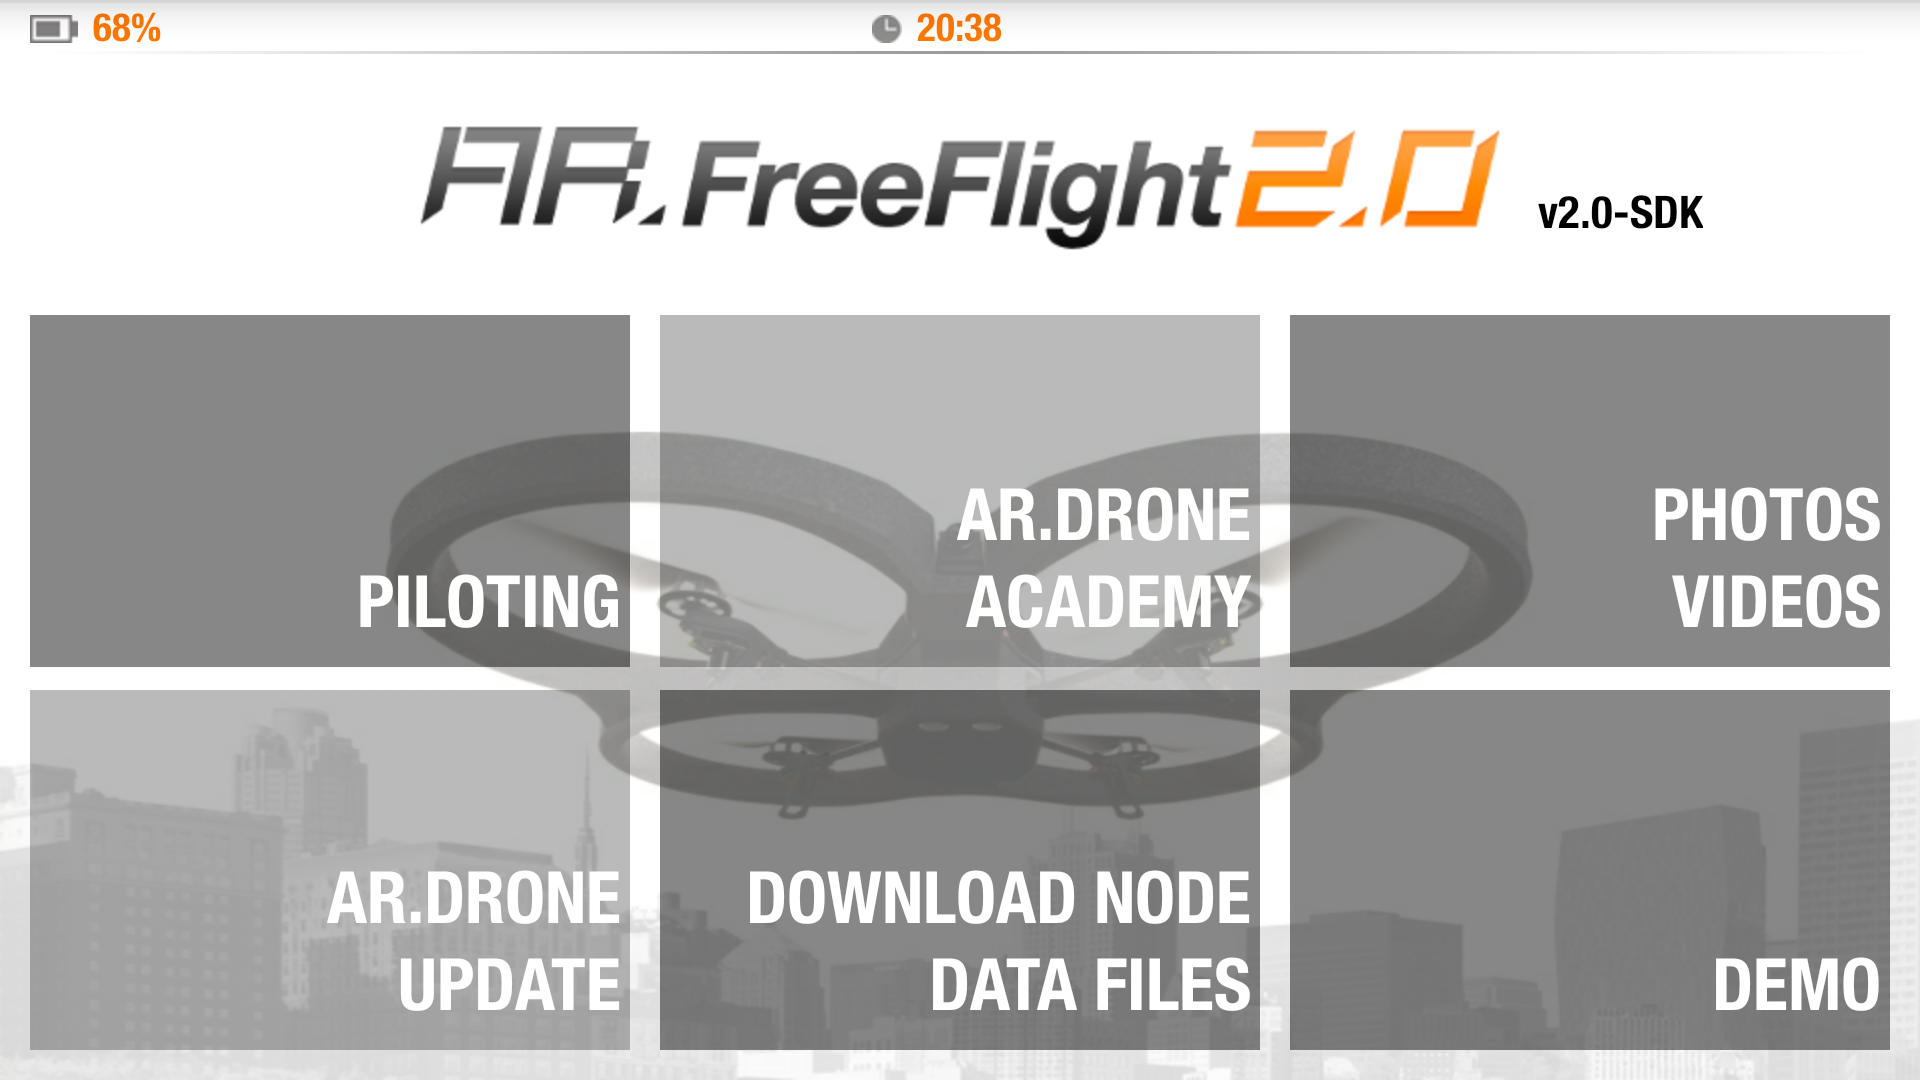
\includegraphics[width=0.9\textwidth]{implementation/android_app.png}
\end{center}
\caption{\small \itshape{ARFreeflight modified application}}
\end{figure}

Being an opensource platform we have moddified the AR Freeflight 2.0 android application to communication with our new modules added tot the drone.

Android fairly imposes the use of the background process class AsynkTask when you have to use communication protocols like http, ftp, sockets. This prevents the ui process from being stuck in communication and not responding to user actions. 

The class offers 5 very important methods that can be overwritten, 3 running on the main ui process and 1 running on the actual background process.

\definecolor{javared}{rgb}{0.6,0,0} % for strings
\definecolor{javagreen}{rgb}{0.25,0.5,0.35} % comments
\definecolor{javapurple}{rgb}{0.5,0,0.35} % keywords
\definecolor{javadocblue}{rgb}{0.25,0.35,0.75} % javadoc
 
\lstset{language=Java,
basicstyle=\ttfamily,
keywordstyle=\color{javapurple}\bfseries,
stringstyle=\color{javared},
commentstyle=\color{javagreen},
morecomment=[s][\color{javadocblue}]{/**}{*/},
numbers=none,
tabsize=4,
showspaces=false,
showstringspaces=false}

\begin{lstlisting}
/* Override this method to perform a computation on a 
background thread.*/
abstract Result	doInBackground(Params... params);
/* Runs on the UI thread after cancel(boolean) is invoked 
and doInBackground(Object[]) has finished. */
void onCancelled(Result result);

/* Runs on the UI thread after doInBackground(Params...). */
void onPostExecute(Result result);

/* Runs on the UI thread before doInBackground(Params...). */
void onPreExecute();

/* Runs on the UI thread after publishProgress(Progress...) 
   is invoked */
void onProgressUpdate(Progress... values);

/* This method can be invoked from doInBackground(Params...) 
   to publish updates on the UI thread while the background 
   computation is still running. */
final void	publishProgress(Progress... values);

\end{lstlisting}

\subsection{Display information module}

\begin{figure}[ht]
\begin{center}
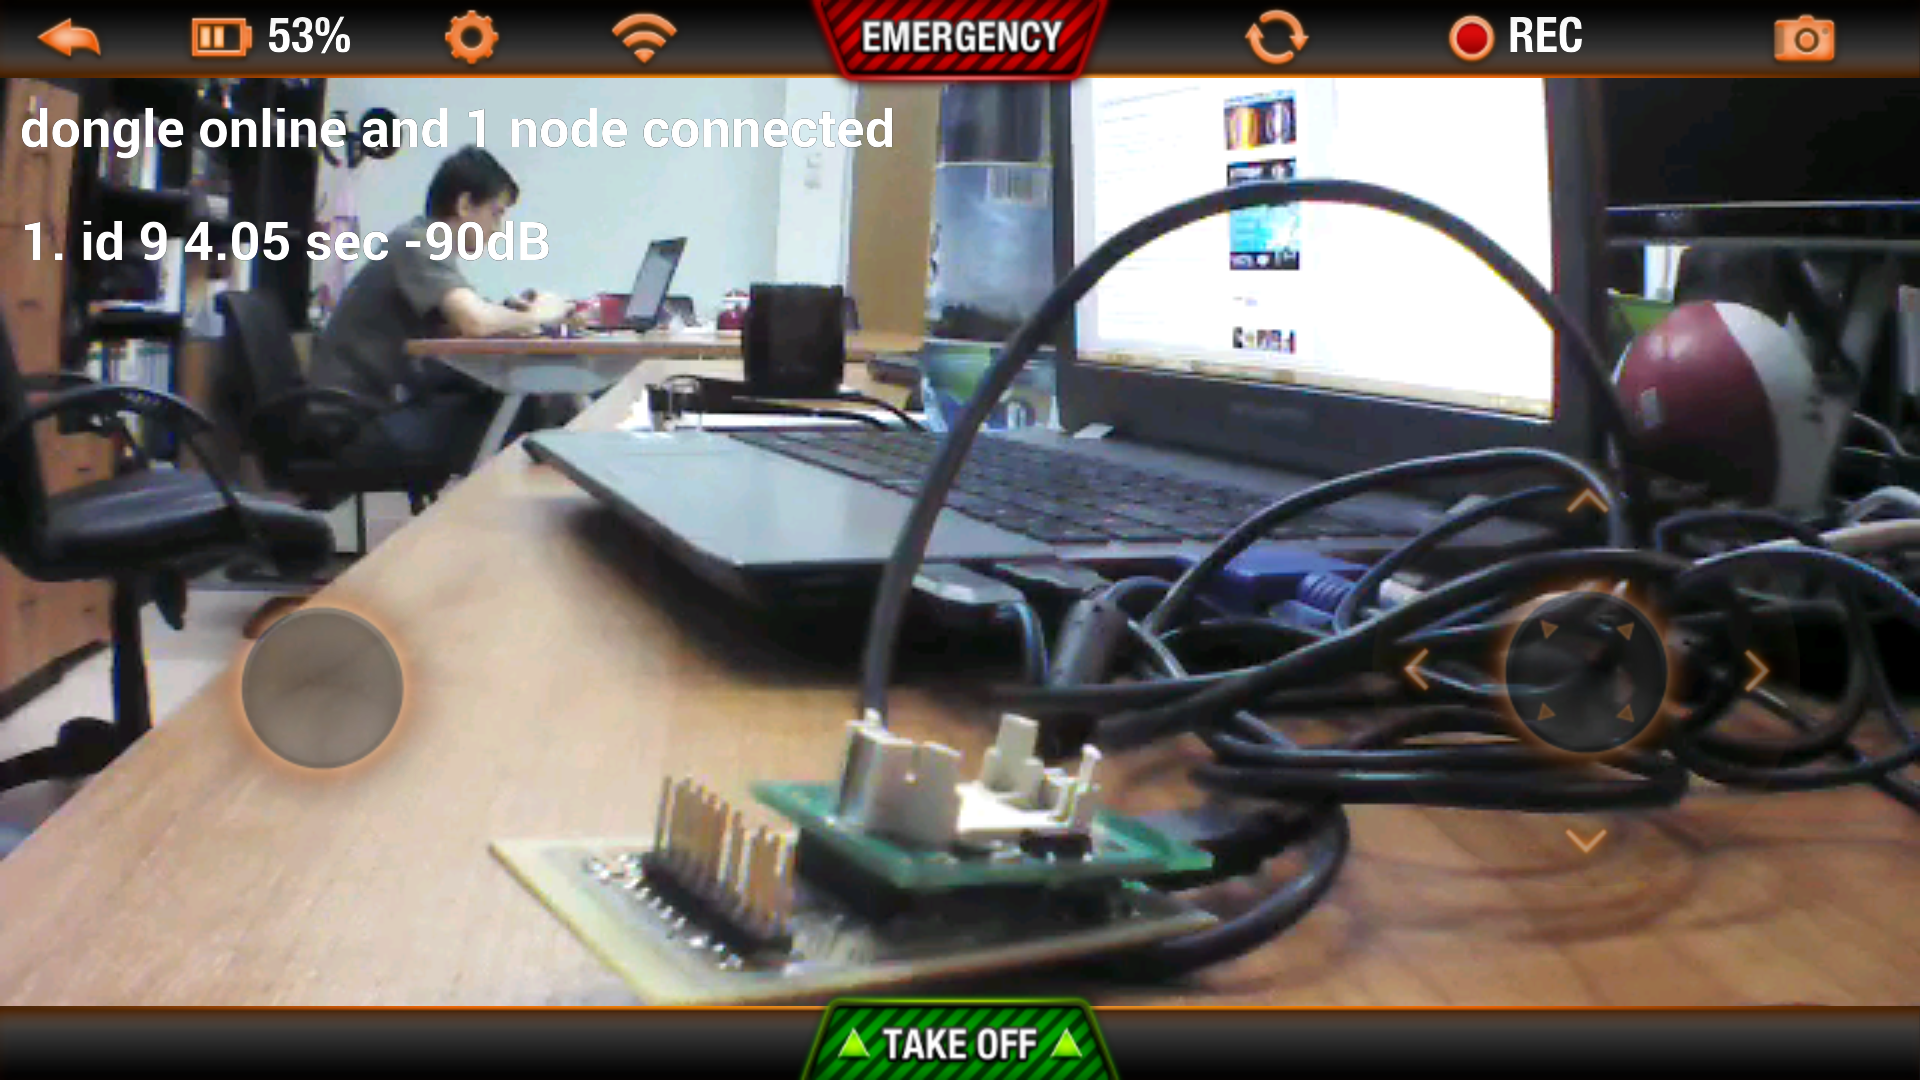
\includegraphics[width=0.9\textwidth]{implementation/android_info.png}
\end{center}
\caption{\small \itshape{ARFreeflight modified Piloting Screen}}
\end{figure}

The Piloting screen of the application has been modified to the display the received informations from the drone. 

The information displayed consists of the dongle being functional and at most, 9 nodes sorted descending after their signal strength. 


\lstset{language=Java,
basicstyle=\ttfamily,
keywordstyle=\color{javapurple}\bfseries,
stringstyle=\color{javared},
commentstyle=\color{javagreen},
morecomment=[s][\color{javadocblue}]{/**}{*/},
numbers=none,
tabsize=4,
showspaces=false,
showstringspaces=false}

\begin{lstlisting}
 
protected void onProgressUpdate(Integer... progress) {
	try {
		// clear the textvies before update
		for (int i = 0; i < txtNodes.length; i++) {
			txtNodes[i].setText("");
		}
		JSONObject jObj = new JSONObject(message);
		JSONArray nodes = jObj.getJSONArray("nodes");
		ArrayList<JSONObject> data = new ArrayList<JSONObject>();
		for (int i = 0; i < nodes.length(); i++) {
			data.add(nodes.getJSONObject(i));
		}
		int dongle_online = jObj.getInt("dongle_connected");
		String txtDongle = "dongle ";
		if (dongle_online == 1) {
			txtDongle += "online";
			txtDongle += " and ";
			if (data.size() == 0) {
				txtDongle += "no nodes connected ";
			} else {
				txtDongle += data.size() + " node";
				if (data.size() > 1) {
					txtDongle += "s";
				}
				txtDongle += " connected";
			}
		} else {
			txtDongle += "offline";
		}
		// first textview is reserved for dongle informations
		txtNodes[0].setText(txtDongle);
		int maxDisplayNodes = data.size();
		// sort data, if there is any
		if (maxDisplayNodes >= 2) {
			Collections.sort(data, new JSONComparator());
		}
		// determine the maximum number of nodes to displat
		if (data.size() > txtNodes.length - 1) {
			maxDisplayNodes = txtNodes.length - 1;
		}
		for (int i = 0; i < maxDisplayNodes; i++) {
			txtDongle = (i + 1) + ". id "
					+ data.get(i).getInt("node_id") + " "
					+ data.get(i).getInt("last_connection_time")
					/ 100.0 + " sec " + data.get(i).getInt("power")
					+ "dB";
			txtNodes[i + 1].setText(txtDongle);
		}
	} catch (Exception e) {
		e.printStackTrace();
	}
}

\end{lstlisting}

\subsection{FTP communication module}

\begin{figure}[ht]
\begin{center}W
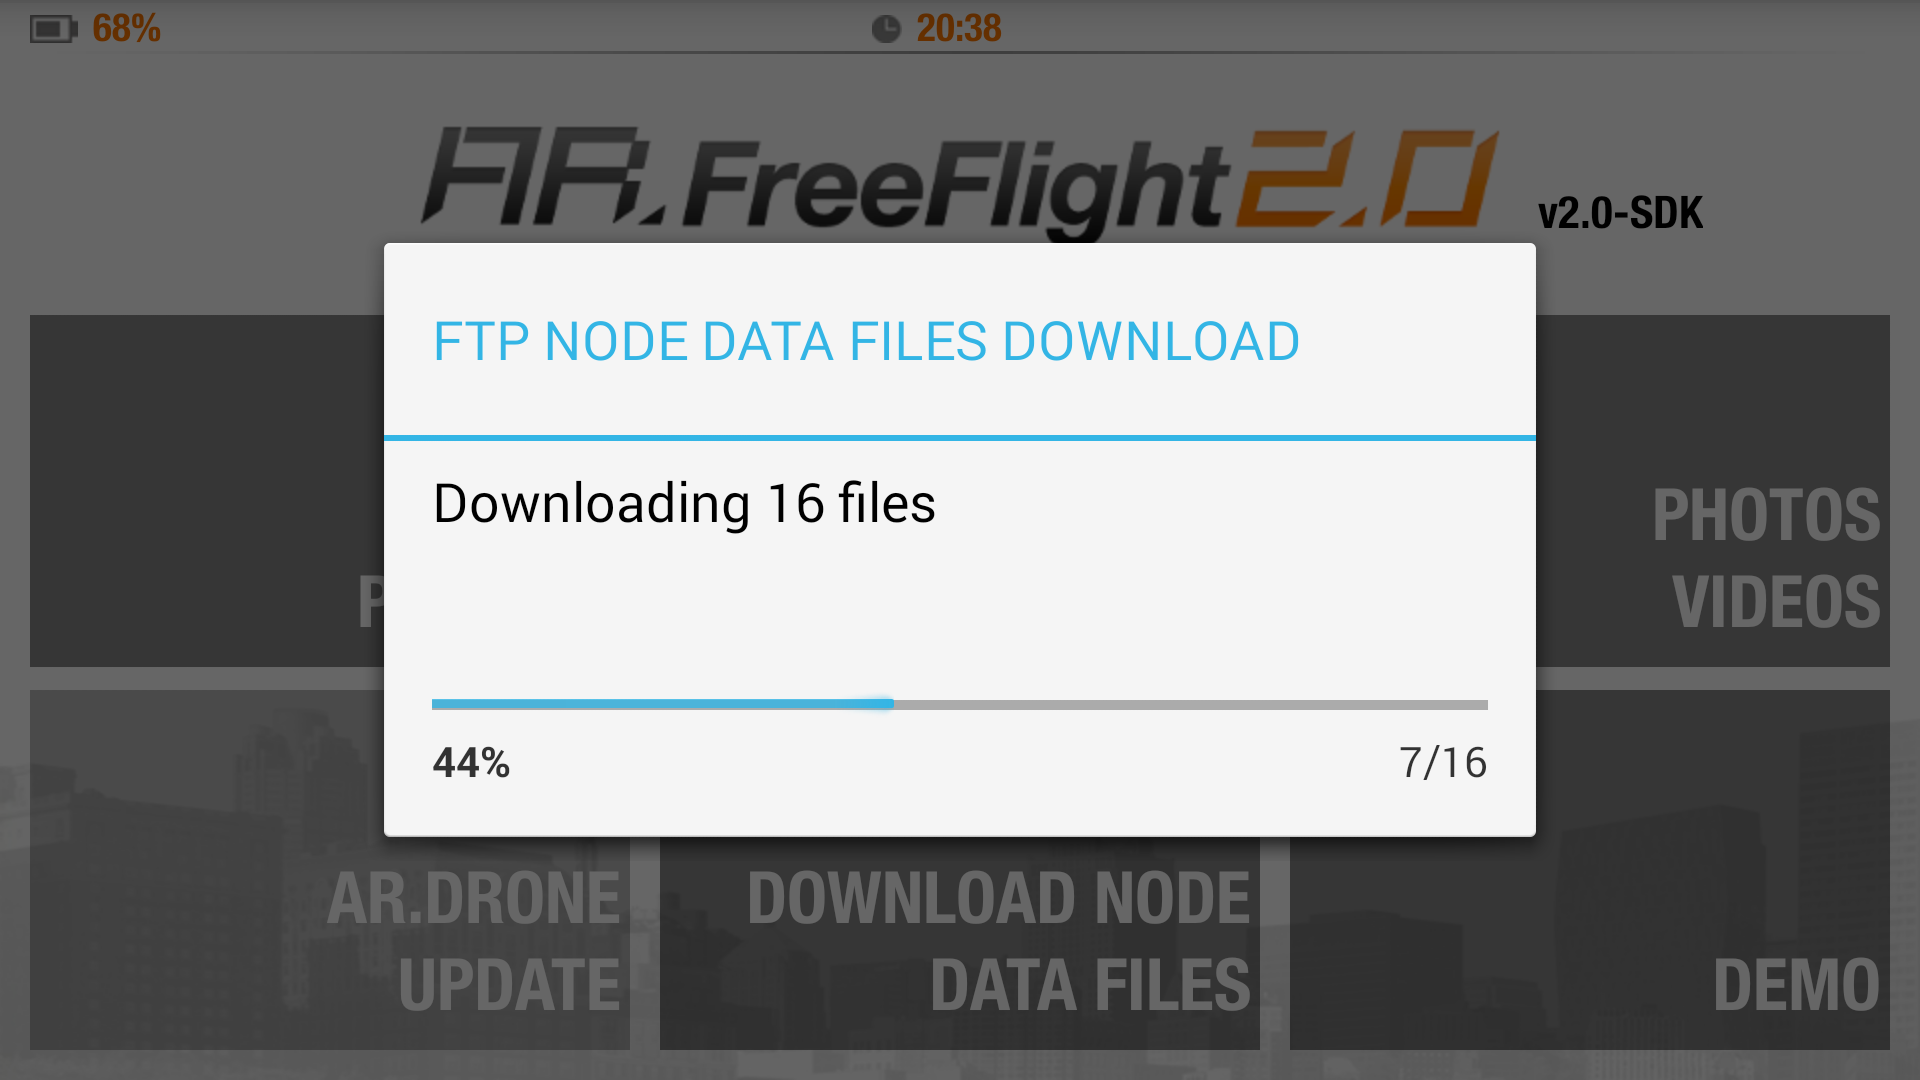
\includegraphics[width=0.9\textwidth]{implementation/android_ftp.png}
\end{center}
\caption{\small \itshape{ARFreeflight FTP downloading files}}
\end{figure}

The drone has a build in FTP server that can be configured to allow acces to any folders/files on the drone. We have configured the drone so that the folder that contains the saved data can be accesed at any time using the 4242 port by any device that has FTP client capabilities. We have added this feature to the android application as well.

The application will download all the files from the drone to the local storage of your android device.

\lstset{language=Java,
basicstyle=\ttfamily,
keywordstyle=\color{javapurple}\bfseries,
stringstyle=\color{javared},
commentstyle=\color{javagreen},
morecomment=[s][\color{javadocblue}]{/**}{*/},
numbers=none,
tabsize=4,
showspaces=false,
showstringspaces=false}

\begin{lstlisting}

protected void onProgressUpdate(Integer... progress) {
	File primaryExtSd = Environment.getExternalStorageDirectory();
	String host = DroneConfig.getHost();
	int port = 4242;
	ftpClient = new FTPClient();
	try {
		ftpClient.connect(host, port);
		FTPFile[] files = ftpClient.listFiles();
		File folder = new File(primaryExtSd, "ftp_node_data");
		folder.mkdir();
		for (int i = 0; i < files.length; i++) {
			File tempFile = new File(folder, files[i].getName());
			ftpClient.retrieveFile(files[i].getName(),
					new FileOutputStream(tempFile));
			publishProgress(new Integer[] { i + 1, files.length });
		}
		return "";
	} catch (Exception e) {
		// TODO Auto-generated catch block
		e.printStackTrace();
	}
	return null;
}
\end{lstlisting}
hfs

